\begin{figure}[bth!]
 \begin{center}
	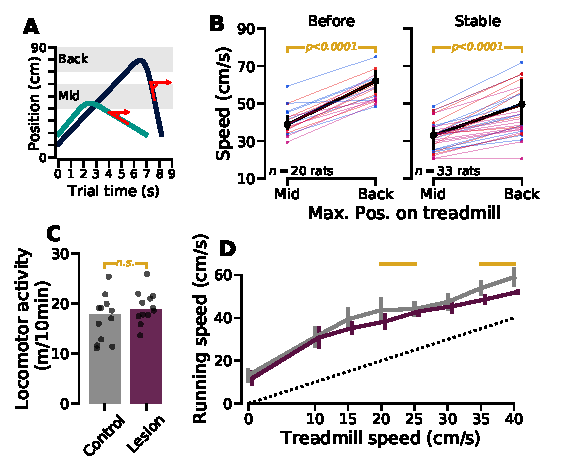
\includegraphics[scale=1]{ch-lesion/figures/MotorPreserved.pdf}
	\caption[Preserved Motor Control After Striatal Lesion]
	{\textbf{Preserved modulation of running speed and spontaneous locomotor activity following striatal lesion.}
	\textbf{(A)} Average speed when rats ran toward the reward area. Data were split according to the position of the rats on the treadmill when initiating their runs.
	\textbf{(B)} Speed of runs initiated either in the back or the middle portion of the treadmill calculated for each animal on the last 5 sessions before lesion (left) and sessions \#4 to \#9 after lesion (right).
	\textbf{(C)} Distance ran while exploring a new immobile treadmill for non-lesioned and lesioned rats ($n=12$).
	\textbf{(D)} Average running speed in a free running task (no reward) in which control and lesioned rats were submitted to trials with incremental treadmill speed (same color code as in C).
	Horizontal golden lines indicated significant differences between groups.
	}
	\label{fig:lesion:motorOk}
 \end{center}
\end{figure}